\documentclass[../main.tex]{subfiles}

\begin{document}

    Más del 99\% de la materia en el universo se encuentra en forma de plasma. Este cuarto estado de la materia se caracteriza por su alto nivel de disociación, en el sentido que la materia se encuentra desligada a nivel atómico. A diferencia de un gas de partículas, en el que la disociación se da a un nivel molecular, en un plasma los electrones se encuentran separados de sus núcleos. Así, tenemos una diversidad de partículas cargadas en su mayoría, conformada por electrones con carga negativa, y los respectivos núcleos o iones con carga positiva, de los que provienen. Aunque el plasma, como un todo, se mantiene eléctricamente neutro, también podemos encontrar en menor cantidad, átomos neutros. En este capítulo, se deducirán cierto parámetros importantes, para la correcta desrcipción de los fenómenos dentro de un plasma, y a sí mismo.

    \section{Apantallamiento de Debye}
        \lhead[\thepage]{\thesection. Apantallamiento de Debye}

    Uno de los efectos básicos, por el cual, se le clasifica a un gas de plasma, es conocido como ``Apantallamiento de Debye". En la superficie
    de la tierra, o a temperatura ambiente, los gases no se encuentran completamente ionizados. Una partícula con carga positiva, por ejemplo,
    situada en la cercanía de la superficie, tiene asociado un campo eléctrico de magnitud igual a
        \begin{align} \label{pot_elec}
            E = \frac{q}{4\pi\epsilon_{0}r^2}.
        \end{align}
    Este campo eléctrico decrece con el inverso del cuadrado de la distancia. Este campo también esta asociado a un potencial eléctrico
        \begin{align}
            &E = -\frac{\partial V(r)}{\partial r}, \\
            &V(r) = \frac{q}{4\pi \epsilon_0 r},
        \end{align}
    donde en el infinito se tiene $V(\infty) = 0$. El efecto de este potencial sobre una partícula cargada es simple, teniendo en cuenta que, las partículas con carga positiva tienden a moverse a potenciales bajos, y las partículas con carga negativa se mueven hacia potenciales altos. La dinámica es relativamente sencilla de estudiar cuando se tienen pocas partículas interactuantes. En un plasma, por el contrario, el potencial eléctrico de las partículas es modificado sutilmente, y surgen otro tipo de fenómenos, producto de tener una mayor densidad del partículas cargadas. \\
    
    Si consideramos las densidades, tanto de electrones como de iones en un plasma, podemos observar que las separaciones entre ambas especies ocurren mínimamente. Las grandes densidades de carga producen fuerzas restaurativas enormes, incluso para distancias relativamente pequeñas de separación. Para un plasma en un reactor, donde se tienen densidades típicas de $10^{20} \ m^{-3}$, podemos imaginar que este desplazamiento provoca que, en un región de cierta longitud, se tenga un exceso de carga o densidad neta positiva (negativa) como en la Figura \ref{fig:figura2.1}. Asumiendo que la densidad sea constante en esa región, e igual a un pequeño porcentaje de la densidad iónica $n_i$, se puede calcular el campo eléctrico en el mismo. Los iones para este caso, al estar acumulados, buscarán moverse hacia afuera, redistribuyendose debido a la repulsión, por lo que, calculando el campo eléctrico, tenemos que
    \begin{align}
        &\vec{\nabla} \cdot \vec E = \frac{\rho}{\epsilon_0}, \\
        &\frac{dE}{dx} = \frac{\rho}{\epsilon_0}, \\
        &E = \frac{\rho}{\epsilon_0}x.
    \end{align}
    \begin{figure}[h] 
        \centering
        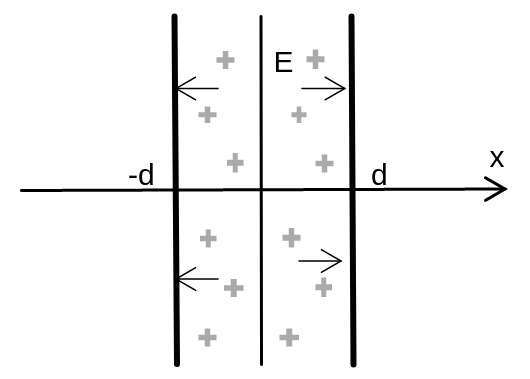
\includegraphics[width=0.5\textwidth]{Images/Debye_shielding.jpg}\caption{Podemos imaginar estos desplazamientos de carga, como pequeñas regiones en el plasma, donde se tiene una exceso de carga igual a una pequeña fracción $\Delta n$ de la densidad total $n.$ }
        \label{fig:figura2.1}
    \end{figure}
    
    Haciendo $x = d = 1 \ cm$, $n_i = 10^{20} \ m^{-3} $ y $\Delta n = 0.01 n_i$, tenemos que
    \begin{align} 
        &F_e = \rho E = \rho^2 \frac{x}{\epsilon_0}, \\
        &F_e = (\Delta ne)^2 \frac{x}{\epsilon_0}, \\
        &F_e = (0.01 \times 10^{20}\   m^{-3}\times 1.6 \times 10^{-19} \ C)^2 \frac{10^{-2} \ m}{8.85 \times 10^{-12} \ C^2\cdot N^{-1}\cdot m^{-2}}, \\
        &F_e \approx 3 \cdot 10^7 \ N \cdot m^{-3}.
    \end{align}

    Debido a la intensa fuerza que experimentan las partículas, producto de esta separación, es que a escala macroscópica, se puede considerar una neutralidad o igualdad de las densidades de electrones e iones a través del plasma. Sin embargo, es importante notar que, esta fuerza decae con la distancia de separación, por lo que, a ciertas longitudes muy pequeñas, la energía interna del plasma, como el movimiento térmico, puede ser suficiente como para mantenerla. Esto no ocurre espontáneamente, debido a que la dinámica de las partículas no es ordenado, sino aleatorio. Sin embargo, existen casos donde esta separación tiene relevancia, sobre todo en la interacción plasma-pared. Este desplazamiento microscópico, da lugar al fenómeno de apantallamiento de Debye, y puede ser estudiado idealmente considerando el potencial eléctrico de un ion estático en el plasma, como en la ecuación (\ref{pot_elec}), y cómo las dem\'as partículas cargadas se distribuyen y ajustan al mismo. Planteando la ecuación de Poisson que relaciona el 
    potencial eléctrico con la densidad de carga 
        \begin{equation}
            \nabla^2\phi = -\frac{\rho}{\epsilon_0}.
        \end{equation}
    Dado que tenemos dos componentes del plasma, sea $n_i$ la densidad de iones y $n_e$ la densidad de electrones locales. La densidad de carga total será
        \begin{equation} \label{2.12}
            \nabla^2\phi =-\frac{(q_in_i+q_en_e)}{\epsilon_0}.
        \end{equation}
    Generalmente, un ion en el plasma tendrá la carga eléctrica igual al número de protones en su núcleo. Considerando núcleos de deuterio (1 protón), y aplicando esto a (\ref{2.12}) tenemos que 
    \begin{align}
        &\nabla^2\phi = -\frac{(en_i-en_e)}{\epsilon_0} \label{2.13}, \\
        &\nabla^2\phi = \frac{e(n_e-n_i)}{\epsilon_0}. \label{2.14}
    \end{align}
    Además asumimos que la densidad de fondo del plasma, para iones, es igual a $n_i$, es decir, tendremos una densidad promedio de iones constante,
    que se distribuye en todo el plasma. Dado que estos iones son mucho más masivos que los electrones, su movilidad será limitada y por ende se puede considerar que solo los electrones son los que se mueven, y cuya densidad varía. Dado que no conocemos la densidad de electrones dentro del plasma, pero que sí se encuentran en equilibro térmico, 
    podemos considerar que los electrones siguen una distribución caracterizada por el factor de Boltzman, según la ecuación
        \begin{equation}
            n_e(r) = n_{0}exp\left(\frac{-q\phi}{k_BT_e}\right).
        \end{equation}
    La densidad $n_0$ es la densidad a distancias muy lejanas, relativamente. A estas distancias, el potencial es pequeño y menos intenso. Y dado
    que el plasma es cuasineutro macroscópica mente, podemos asumir que en estas zonas la densidad de electrones será igual a la densidad
    promedio de fondo de los iones $n_i$ 
    \begin{align}
        &n_i(r) = n_0, \label{equ2.16} \\ 
        &n_e(r) = n_iexp\left(\frac{-q\phi}{k_BT_e}\right).
    \end{align}
    Considerando además la aproximación 
        \begin{equation} \label{equaprox} \frac{e\phi}{k_BT_e} << 1,
        \end{equation}
    podemos expandir el exponencial y tomar los términos de primer orden
        \begin{equation} exp(\frac{e\phi}{k_BT_e}) \approx 1 + \frac{e\phi}{k_BT_e},
        \end{equation}
    y reemplazando en (\ref{2.14}) 
    \begin{align}
        &\nabla^2\phi = \frac{e(n_i+n_i(e\phi/k_BTe)-n_i)}{\epsilon_0}, \\
        &\nabla^2\phi = \frac{e^2n_i}{k_BT_e\epsilon_0}\phi.
    \end{align}
    Si asumimos una simetría esférica para el potencial, tenemos que 
        \begin{equation}
            \frac{1}{r^2}\frac{d}{dr}(r^2\frac{d\phi}{dr}) = \alpha^2\phi,
        \end{equation}
    donde
        \begin{equation}
            \alpha^2 = \frac{e^2n_i}{k_BT_e\epsilon_0}.
        \end{equation}
    Reacomodando factores
        \begin{equation}
            \frac{d^2}{dr^2}(r\phi) = \alpha^2(r\phi),
        \end{equation}
    por lo que, para el potencial, tenemos que
        \begin{equation} \label{2.25}
            \phi = \frac{A}{r}exp^{-\frac{r}{\lambda_D}},
        \end{equation}
    donde
        \begin{equation}
            \lambda_D = \frac{1}{\alpha} = (\frac{k_BT_e\epsilon_0}{e^2n_i})^{1/2},
        \end{equation}
    y de (\ref{equ2.16})
        \begin{align}
            \lambda_D = (\frac{k_BT_e\epsilon_0}{e^2n_0})^{1/2}. \label{long_deby}
        \end{align}
        
    Lo que nos dice el resultado (\ref{2.25}) es que, el potencial eléctrico de una carga positiva en el plasma (de igual manera se puede tomar el caso 
    para un electrón) es cancelado o ``apantallado" más allá de cierta longitud $\lambda_D$, como se observa en la Figura (\ref{fig:apantallamiento}) . Los electrones siguen la distribución considerada debido al potencial generado por el ion. Los electrones serán atraídos, mientras que los iones circundantes serán repelidos, aunque en un menor grado, debido a la suposición de su movilidad.   Sin embargo, esto no quiere decir que los iones estén completamente 
    inmóviles. Estás partículas también experimentan interacciones, y se puede tomar una distribución correspondiente
    para estas partículas. \\

%%%%%%%%%%%%%%%%%%%%%%%%%%%%%%%%%
\begin{comment}
    

    Dado que el potencial eléctrico es más intenso cerca del ión 
    positivo, los electrones tenderán a juntarse cerca del mismo, mientras que los iones se alejarán, cambiando ambas densidades. Más allá
    de cierta longitud, el potencial eléctrico es muy débil y la densidad de electrones es pequeña.\\
    
    Este comportamiento impide que los electrones se acumulen excesivamente alrededor del ión. Así, cada partícula siente el campo de las partículas 
    dentro de esta pequeña región determinada por la longitud característica, más no de las que están fuera, pues esos campos son ''apantallados" 
    por este fenómeno.\\
\end{comment}
%%%%%%%%%%%%%%%%%%%%%%%%%%%%%%%%%
    \begin{figure}[h] 
        \label{fig:apantallamiento}
        \centering
        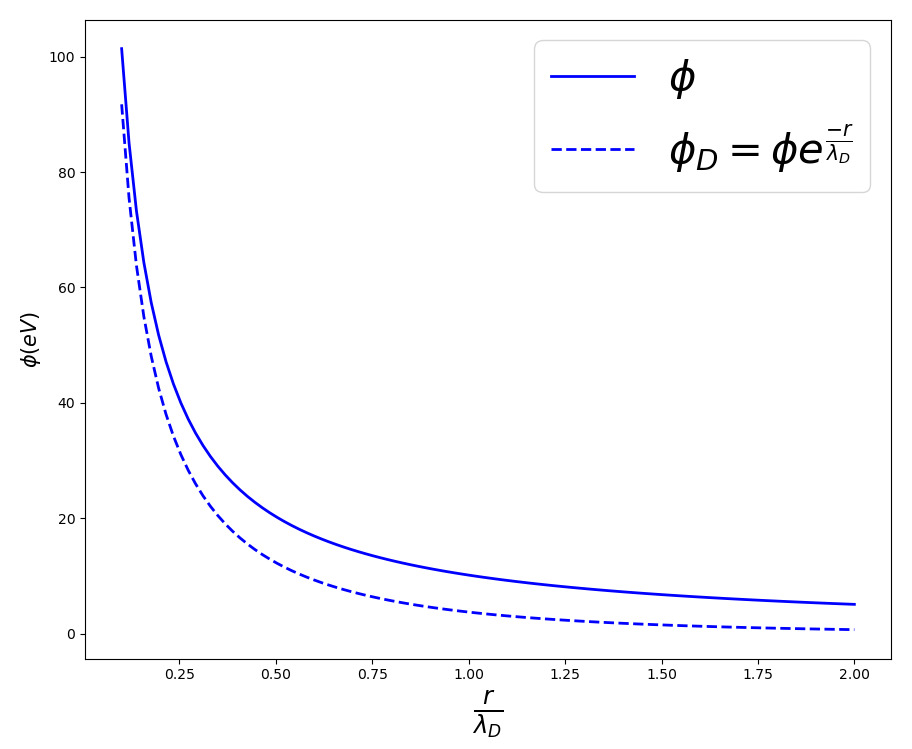
\includegraphics[width=0.9\textwidth]{Images/Potencial_modificado.jpg}
        \caption{Potencial Apantallado $\phi_D$. Se puede observar que el potencial de la carga es reducido o apantallado más allá de cierta longitud $\lambda_D$. La influencia más allá de esta longitud ya no es relevante, y se considera que, la carga solo interactúa con aquellas que estan más cerca o una distancia menor que $\lambda_D$.}
        \label{fig:apantallamiento}
    \end{figure}

    Además, la temperatura asumida en los cálculos, es la temperatura asociada a los electrones, es decir, se asume que durante el tiempo que duró
    el proceso de estudio, las partículas positivas (iones) y negativas (electrones) estuvieron en equilibrio térmico y alcanzaron las temperaturas
    $T_i$ y $T_e$ respectivamente (ambas especies estuvieron en equilibrios térmicos distintos). Dado que los electrones tienen más movilidad,
    estos tienen más responsabilidad al momento de moverse y crear regiones con más o menos carga negativa. Esto no significa que ambas especies no puedan alcanzar el equilibrio térmico conjunto. Depende del tiempo durante el cual, el plasma exista,
    lo que determinará cómo evoluciona la temperatura del sistema. Si se toma en cuenta que ambas especies están en equilibrio térmico, es decir, están a una misma temperatura, y considerando para ambas, distribuciones 
    de Boltzman para sus densidades, el cálculo anterior muestra que el apantallamiento sufre un pequeño cambio, no relevante, respecto de la 
    manera en que el potencial decae, lo cual como sería de esperarse, tendría que caer un poco más rápido. Para el caso descrito, no se asumiría una densidad promedio de fondo para los iones, sino más bien, para distancias más lejanas, ambas densidades se 
    igualarían a un $n_0$ y volverían al plasma cuasineutro. Se debe tomar en cuenta que,  cuando se alcanza el equilibrio térmico total entre todas las especies, para los iones 
    con poca movilidad, la componente del apantallamiento debida a los electrones, tiene más contribución que la componente debida a los iones,
    mientras  que para los electrones con mucha movilidad, la componente del apantallamiento debido a los electrones es baja, mientras que la 
    componente debida a los iones es casi nula.\\
    
    Podemos decir entonces que, la intensidad de este potencial apantallado tendrá relevancia hasta esta longitud característica. Por lo tanto, cada carga interactúa solo con las partículas dentro de una región limitada por la longitud de Debye. Esta región es denominada también esfera de Debye, cuyo radio será igual a $\lambda_D$. Podemos entonces, calcular el número de partículas dentro de esta esfera, como
\begin{align}
&N_D = \frac{4}{3}\pi \lambda_D^3 n_0, \label{N_D} \\
&N_D = \frac{4}{3}\pi \left( \frac{k_BT_e\epsilon_0}{e^2n_0^{1/3}}\right)^{3/2}
\end{align}
Como se mencionó anteriormente, para que se exhiba este comportamiento colectivo dentro del plasma, es necesario que haya cierto número de partículas al interior de la esfera de Debye, es decir, debe ser mucho mayor que uno. Además, también debe considerarse que, las dimensiones del sistema $L$ deben ser mucho mayores que $\lambda_D$. Estas consideraciones sirven como criterios para poder definir a lo que llamamos plasma, y que se puedan manifestar las interacciones colectivas características. \\

 \begin{figure}[h]
        \centering
        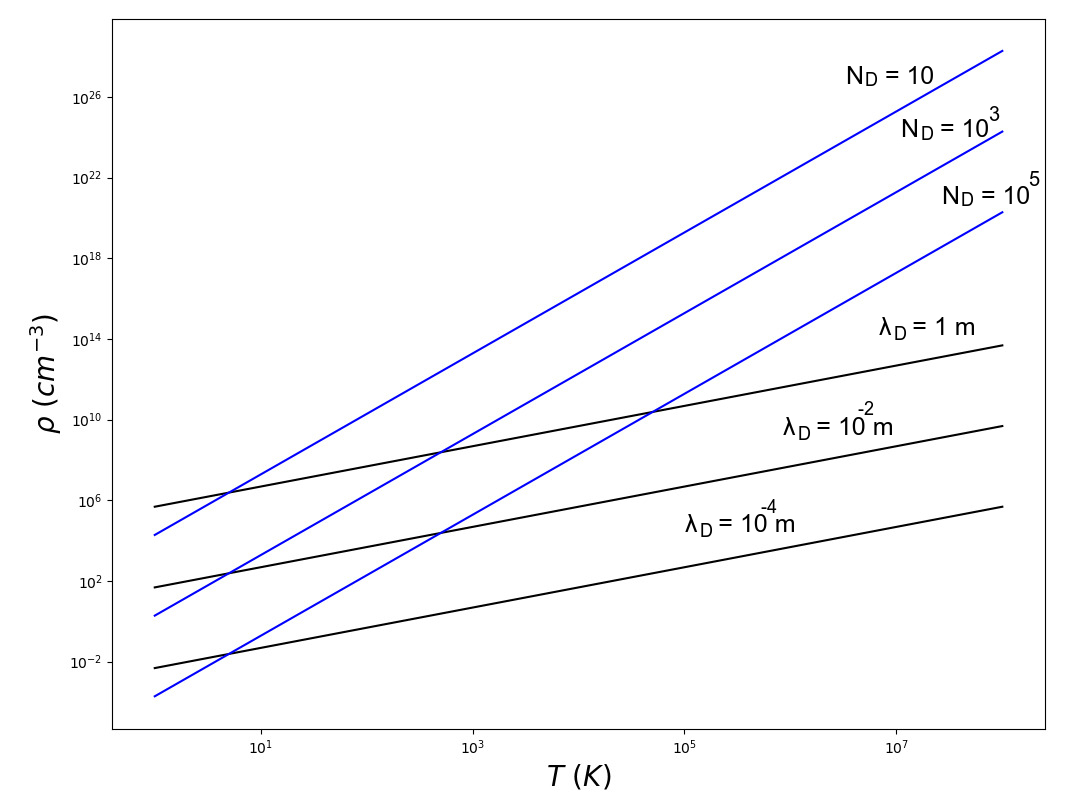
\includegraphics[width=0.8\textwidth]{Images/long_part.jpg}
        \caption{Algunos valores para $\lambda_D$ y $N_D$.}
    \end{figure}
    Otro caso es en el que, se consideran dos equilibrios térmicos correspondientes a cada especie.
    Asociamos entonces una temperatura $T_e$ para los electrones, y una temperatura $T_i$ para los iones, donde ahora, se considerará que la movilidad de los mismos ya no es limitada. Por lo tanto, para cada especie tenemos que la distribución de densidades será
        \begin{align}
            &n_e(r) = n_0exp\left(\frac{e\phi}{k_BT_e}\right), \\
            &n_i(r) = n_0exp\left(\frac{-e\phi}{k_BT_i}\right),
        \end{align}
    donde $n_0$ es la densidad promedio constante para ambas especies a grandes distancias, donde se supone que el plasma es cuasineutro. Ahora, usando la aproximación (\ref{equaprox}) 
        \begin{align}
             &n_0exp\left(\frac{e\phi}{k_BT_e}\right) \approx n_0\left(1+\frac{e\phi}{k_BT_e}\right), \\
             &n_0exp\left(\frac{-e\phi}{k_BT_e}\right) \approx n_0\left(1-\frac{e\phi}{k_BT_i}\right).
        \end{align}
    Reemplazando ambas distribuciones en (\ref{2.14}) tenemos
        \begin{align}
            &\nabla^2\phi = \frac{e(n_0+n_0(e\phi/k_BT_e)-n_0+n_0(e\phi/k_BT_i))}{\epsilon_0}, \\
            &\nabla^2\phi = \left(\frac{n_0e^2}{k_B\epsilon_0T_e} + \frac{n_0e^2}{k_B\epsilon_0T_i}\right)\phi,
        \end{align}
    en donde definimos la longitud de Debye como
        \begin{equation}
            \lambda_T=  \left(\frac{n_0e^2}{k_B\epsilon_0T_e} + \frac{n_0e^2}{k_B\epsilon_0T_i}\right)^{-\frac{1}{2}}.
        \end{equation}
    Tenemos entonces que, esta es la longitud característica del apantallamiento del potencial eléctrico, según las nuevas consideraciones hechas. A este tipo de plasmas se les conoce como plasmas no térmicos, debido a que sus componentes se encuentran a distintas temperaturas. Si el plasma se sostiene lo suficiente para que ambas especies entren en un equilibrio térmico total, a una temperatura $T$, entonces las 
    temperaturas usadas en las distribuciones respectivas, son reemplazadas por esta nueva temperatura. Siguiendo los cálculos anteriores, tenemos
    que
        \begin{align}
            &\nabla^2\phi = \frac{e(n_0+n_0(e\phi/k_BT)-n_0+n_0(e\phi/k_BT))}{\epsilon_0}, \\
            &\nabla^2\phi = (\frac{2n_0e^2}{k_B\epsilon_0T})\phi.
        \end{align}
    La longitud de Debye correspondiente será
        \begin{equation}
            \lambda_D=  \left(\frac{2n_0e^2}{k_B\epsilon_0T}\right)^{-\frac{1}{2}}.
        \end{equation}
    A este tipo de plasmas se le conoce como plasma térmico, debido a que se llega a un equilibrio térmico total.


    \section{Frecuencia del plasma}
     \lhead[\thepage]{\thesection. Frecuencia del plasma}

    La neutralidad macroscópica del plasma, permite que no se generen desviaciones considerables en las densidades, que alteren el sistema e introduzcan campos eléctricos que puedan perturbar las poblaciones de partículas circundantes. Sin embargo, cuando se asume cierto desplazamiento en la densidad de carga, la dinámica de las partículas cambia, debido a los campos
    eléctricos generados por estas distribuciones netas de carga eléctrica. Para entender esto, tomemos una región neutra dentro del plasma. Dentro de esta región tendremos densidades de electrones e iones (núcleos),
    que en conjunto dotan de esta neutralidad a esta región. Si desplazamos la densidad de electrones hacia la derecha, entonces tendríamos
    una región polarizada que origina un campo eléctrico como se muestra en la Figura \ref{fig:frecuencia_plasmas}.

        % Introducir aquí la imagen
        \begin{figure}[h]
        \centering
        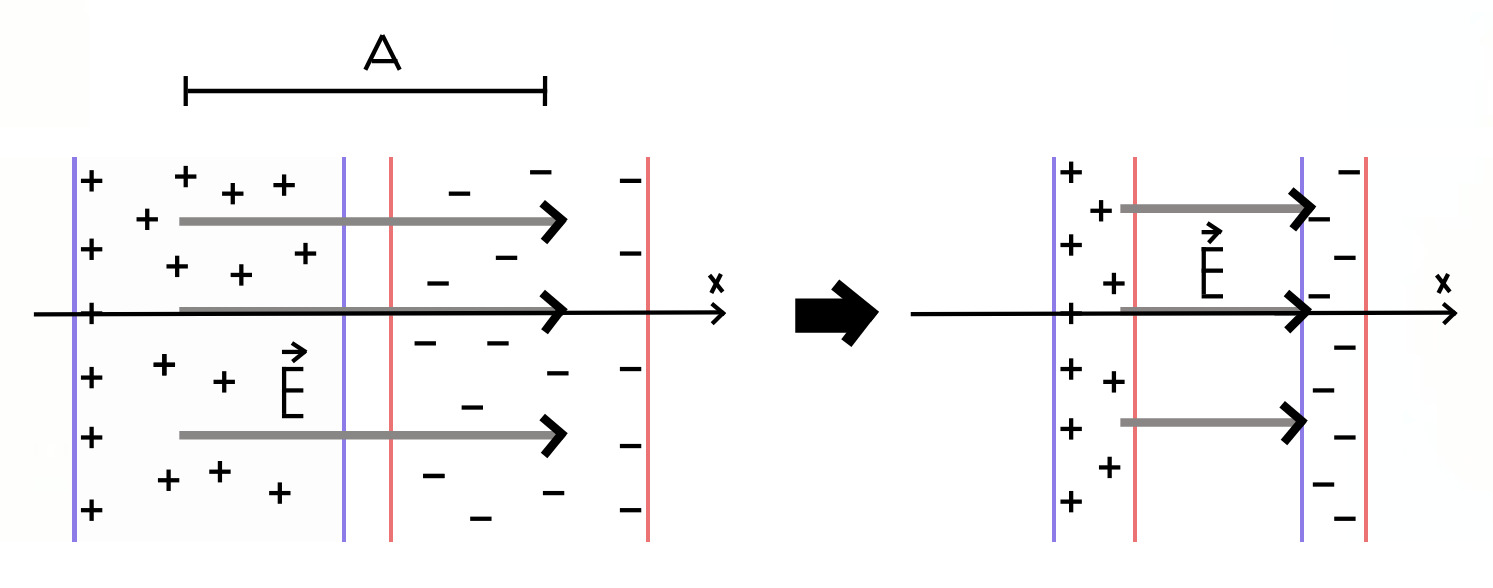
\includegraphics[width=17cm,height=7cm]{Images/frecuencia_plasmas.jpg}
        \caption{Desplazamiento de las densidades de carga. Este exceso de carga negativa a la derecha, puede ser visto como una pequeña perturbación introducida dentro del plasma. Se asume una separación promedio de longitud $A$ o amplitud de oscilación muy pequeña.}
        \label{fig:frecuencia_plasmas}
        \end{figure}

    Entonces, para estudiar este fenómeno, asumimos una pequeña perturbación en esta región \cite{chen1984introduction}, que tiene la forma de un plano infinito de cierto grosor no relevante. Dado que esta región proviene de haber desplazado una densidad de carga negativa de otra región, tendremos una región analoga a esta pero con una densidad de carga positiva neta. Esta configuración de cargas intuye a pensar en un comportamiento oscilatorio, pues los electrones sentirán el campo eléctrico resultante
    y se moverán en dirección contraria a él. Asumiendo también, que el movimiento solo se da a lo largo del eje x, para esta región en donde hemos introducido la perturbación, tomamos las siguiente cantidades
        \begin{align}
            &n_e(x,t) = n_0 + \tilde{n}_e(x,t), \label{perturbacion}\\
            &v_e(x,t) = v_{e0} + \tilde{v}_e(x,t), \\
            &E(x,t) = E_0 + \tilde{E}(x,t),
        \end{align}
    donde $v_e$ es la velocidad promedio de los electrones y $E$ el campo eléctrico al interior del plasma. El primer término de la parte derecha para cada ecuación, representa la parte no perturbada de cada magnitud, mientras que el segundo término es la parte perturbativa. Para simplificar más nuestro modelo, asumiremos que no hay movimiento térmico alguno, o en otras palabras, $T = 0$. Por lo tanto, inicialmente se tiene $v_{e0} =0$. En (\ref{perturbacion}), $n_0$ es la densidad inicial, y está asociada a la neutralidad del plasma, que hace que en el interior, $E_0 = 0$. Asumiendo que el comportamiento oscilatorio se manifiesta también en la velocidad promedio y en el campo eléctrico, tenemos
        \begin{align}
            &\tilde{n}_e(x,t) = Af_1(kx - \omega_et), \\
            &\tilde{v}_e(x,t) = Bf_2(kx - \omega_et), \label{velocidad_perturbada}\\
            &\tilde{E}_e(x,t) = Cf_3(kx - \omega_et), \label{campo_perturbado}
        \end{align}
    en donde $f_i$ es una función periódica con frecuencia $\omega_e$, y amplitudes $A, \ B, \ C << 1$. Básicamente, estas perturbaciones oscilarán con una amplitud muy pequeña, lo que refleja también la magnitud de nuestra perturbación. Luego, la densidad de carga eléctrica neta será la suma de la densidad eléctronica e iónica. Consideramos que los iones son mucho más masivos que los electrones, por lo que su respuesta a las oscilaciones eléctronicas son lentas, y la variación en su densidad, en primera aproximación, se puede despreciar, o considerarlos cuasiestáticos. Entonces
        \begin{align}
            &\rho = -en_e+en_i, \\
            &\rho = -en_e+en_0, \\
            &\rho = -e(n_0 + \tilde{n}_e(x,t)) + en_0, \\
            &\rho = -e\tilde{n}_e(x,t).
        \end{align}
    Debido a esta densidad de carga eléctrica, se generará un campo eléctrico resultante y la cantidad de momento lineal cambiará debido a este, acelerando o desacelerando a las partículas. También aplicamos la ecuación de continuidad sobre la región inicialmente neutra, dado que tenemos una densidad electrónica que varía, debido al flujo de partículas sobre la región considerada. Tomando la velocidad promedio $\vec{v}_e$ para los electrones, tenemos que la ecuación para el campo eléctrico, para la conservación del momento lineal, y la ecuación de continuidad para las partículas son respectivamente
        \begin{align}
            &\nabla \cdot \vec{E} = \frac{\rho}{\epsilon_0}, \label{gauss}\\
            &m_en_e \left( \frac{\partial \vec{v}_e}{\partial t} + (\vec{v}_e \cdot \nabla)\vec{v}_e \right) = -en_e\vec{E}(x,t), \label{equ2.51}\\
            &\frac{\partial n_e(x,t)}{\partial t} + \nabla \cdot (n_e\vec{v}_e) = 0. \label{continuidad}
        \end{align}
        Usando la ecuación (\ref{perturbacion}) en (\ref{continuidad}) tenemos que
        \begin{align}
            &\frac{\partial \left(n_0 + \tilde{n}_e(x,t)\right)}{\partial t} + \nabla \cdot [(n_0+\tilde{n}_e)\vec{v}_e]= 0.
        \end{align}
    Los productos $\tilde{n}_e\vec{v}_e$, y $(\vec{v}_e \cdot \nabla)\vec{v}_e$ en (\ref{equ2.51}), tienen una amplitud de segundo orden, debido a (\ref{velocidad_perturbada}) y (\ref{campo_perturbado}), el cual despreciamos para efectos de cálculo. Entonces
        \begin{align}
            &\frac{\partial \tilde{n}_e(x,t)}{\partial t} + n_0\nabla \cdot \vec{v}_e(x,t) = 0, \label{equ2.54}\\
            &m_e \left( \frac{\partial \vec{v}_e}{\partial t} \right) = -e\vec{E}
            (x,t). \label{equ2.55}
        \end{align}
    Ahora, aplicando el operador de divergencia en (\ref{equ2.55}) y usando (\ref{gauss})
        \begin{align}
            &m_e\frac{\partial}{\partial t}\nabla \cdot \vec{v}_e(x,t) = -e\nabla \cdot \vec{E}(x,t), \\
            &m_e\frac{\partial}{\partial t}\nabla \cdot \vec{v}_e(x,t) = \frac{e^2}{\epsilon_0}\tilde{n}_e(x,t). \label{equ2.57}
        \end{align}
    Despejando $\nabla \cdot \vec{v}_e$ en (\ref{equ2.54}) y reemplazando en (\ref{equ2.57})
        \begin{align}
            &m_e\frac{\partial}{\partial t}\left( -\frac{1}{n_0} \frac{\partial \tilde{n}_e(x,t)}{\partial t} \right) = \frac{e^2}{\epsilon_0}\tilde{n}_e(x,t), \\
            &\frac{\partial^2 \tilde{n}_e(x,t)}{\partial t^2} + \left( \frac{e^2n_0}{m_e\epsilon_0} \right) \tilde{n}_e(x,t) = 0. \label{equ2.59}
        \end{align}
        
    La ecuación anterior tiene por solución, funciones periódicas como habíamos asumido. Observamos que esta perturbación oscila alrededor de la región considerada, debido al campo eléctrico producido por la misma. Los electrones, al ser separados de su posición de equilibrio, son atraídos por el campo eléctrico resultante. Estos aceleran hasta que vuelven a las condiciones iniciales, pero la inercia de su movimiento hace que sigan moviéndose hasta que el campo se invierta y, nuevamente se repite el proceso. La frecuencia de estas oscilaciones se deduce directamente de la ecuación (\ref{equ2.59})
        \begin{align}
            &\frac{\partial^2 \tilde{n}_e(\vec{r},t)}{\partial t^2} + \omega_e^{2} \tilde{n}_e(\vec{r},t) = 0 \\
            &\omega_e = \left( \frac{e^2n_0}{m_e\epsilon_0} \right)^{1/2}.
        \end{align}
        
    Observamos que la frecuencia es directamente proporcional a la raíz cuadrada de la densidad inicial. Para estimar esta frecuencia, asumimos
    un plasma con una densidad $n_0 = 10^{20} m^{-3}$, tenemos entonces
    $\omega_e \approx 10^{11} rad/s$. Dado que, en un plasma también existe cierta densidad de átomos neutros, estas oscilaciones también están sujetas a efectos de amortiguación. Entonces, si denotamos por $t_{ea}$ el tiempo promedio entre colisiones electrón-átomo, y $t_e$ el periodo de oscilación, tenemos que la frecuencia de oscilación $\omega_e$ debe satisfacer
    \begin{align}
        t_e &< t_{ea}, \\
        \frac{1}{t_{ea}} &< \frac{1}{t_e}, \\
        \frac{1}{t_{ea}} &< \nu_e,\\
        1 &< t_{ea}\omega_e,
    \end{align}
    Donde $\nu_e = \omega_e / 2\pi$. Para que el plasma pueda experimentar cambios apreciables en el valor de sus parámetros, el tiempo promedio entre colisiones debe ser lo suficientemente grande como para evitar que las amortiguaciones hagan que los electrones se acoplen al equilibrio de los átomos neutros \cite{bittencourt2013fundamentals}. De está manera se logra un comportamiento independiente para los electrones.
    
        
    \section{Parámetro del plasma}
    \lhead[\thepage]{\thesection. Parámetro del plasma}
    
    La gran cantidad de fenómenos que surgen al interior de un plasma, son debido a las interacciones electromagnéticas entre las partículas cargadas. Sin embargo, dado que se tiene un grán número de ellas a determinada temperatura $T$, se tiene que tener en cuenta la naturaleza estadística del sistema. Podemos estimar cual es la naturaleza predominante dentro de un plasma, y que definirá el modo de estudio del mismo. De manera sencilla, consideremos dos partículas con la misma carga y signo $q$. Tomando como marco de referencia una de ellas, suponemos que la otra partícula se acerca a ella con una velocidad relativa $v$ y con una energía cinética determinada. Además, debido a su naturaleza eléctrica, el sistema irá acumulando energía potencial eléctrica, a medida que se acerquen. Entonces, para este pequeño sistema, tenemos que la energía total es
\begin{align}
	E(r,v) = \frac{1}{2}mv^2 - \frac{q^2}{4\pi\epsilon_0 r}.
\end{align}

Podemos definir una distancia de máximo acercamiento, donde toda la energía cinética se transforme en energía potencial eléctrica. Aquí, la energía total $E$, será igual a cero. Denotamos como $d_a$ a esta distancia, y tomando la energía cinética, igual a la energía térmica $k_B T$, tenemos que
\begin{align}
	&E(d_a,v_a) = 0, \\
	&\frac{1}{2}mv_a^2 = \frac{q^2}{4\pi\epsilon_0 d_a}, \\ 
	&k_BT = \frac{q^2}{4\pi\epsilon_0 d_a}, \\
	&d_a = \frac{q^2}{4\pi\epsilon_0 k_BT}. \label{r_a}
\end{align}
Otra longitud importante que considerar, es la distancia media entre partículas $d_m$, la cual puede ser definida por medio de la densidad $n$ del sistema como
\begin{align}
    d_m \equiv \frac{1}{n^{1/3}}. \label{d_m}
\end{align}
Podemos concebir intuitivamente $d_m$, como la longitud de uno de los lados de un cubo de volumen igual al de una partícula en el sistema. El volumen, en este caso, sería igual a la inversa de la densidad, $1/n$. Ahora, de (\ref{r_a}), podemos observar que, mientras mayor sea la temperatura dentro de un plasma, menor sera la distancia de máximo acercamiento, y visceversa. Entonces, tomando de referencia la distancia media entre partículas (\ref{d_m}), que está en función de la densidad del plasma, podemos decir que las interacciones eléctricas serán predominantes si $d_m < d_a$. Esto es debido a que la energía térmica no es suficiente para poder sobrepasar a la energía potencial eléctrica del sistema, más allá de la longitud $d_m$, que como hemos dicho, se toma como distancia de referencia o normal. Por otro lado, si la temperatura es lo suficientemente alta como para que la energía térmica sobrepase a la potencial eléctrica más allá de $d_m$, entonces $d_a < d_m$, y las partículas se aproximarán más que la distancia que los separa en promedio. Dado que las interacciones eléctricas pueden tener o no, mayor grado de relevancia dentro de un plasma, y que la dinámica de una partícula está influenciada por la de las demás, en este sentido, decimos que se puede tener un plasma fuertemente acoplado si $d_m < d_a$, o debilmente acoplado si $d_a < d_m$. El concepto de acoplamiento, tiene que ver con la evolución de cada partícula en el plasma y su dependencia dinámica con las demás. Es por esta razón, que la complejidad para resolver las ecuaciones de movimiento, de sistemas de muchos componentes con estás interacciones (eléctrica), es enorme.\\

El acoplamiento en el plasma también puede ser descrito utilizando otra magnitud adimensional, denominada parámetro del plasma, el cual es análoga a $N_D$ en (\ref{N_D}) salvo por un factor de $1/3$. Se define como
\begin{align}
    \Lambda = 4\pi n\lambda_D^3,
\end{align}
y depende de $d_m$ y $d_a$, reemplazando (\ref{long_deby}) y teniendo en cuenta que $k_B\epsilon_0T/e^2n =1/4\pi d_an$
\begin{align}
    &\Lambda = 4\pi n\left(\frac{k_B\epsilon_0T}{e^2n}\right)^3, \label{Lambda_Tn} \\
    &\Lambda = 4\pi n\left(\frac{1}{4\pi d_an}\right)^{3/2}, \\
    &\Lambda = \frac{1}{\sqrt{4\pi}}\frac{1}{n^{1/2}}\left(\frac{1}{d_a}\right)^{3/2}, \\
    &\Lambda = \frac{1}{\sqrt{4\pi}}\left(\frac{d_m}{d_a}\right)^{3/2},
\end{align}
donde $d_m^{3/2}= 1/n^{1/2}$. Si $d_m << d_a $, entonces $\Lambda << 1$. En este caso el acoplamiento será mayor y las interacciones eléctricas harán que se tengan pocas partículas en una esfera de Debye (considerando que $\Lambda = N_D/3$). Si $d_a << d_m$, entonces $\Lambda >> 1$. Luego, se tendrán más partículas en una esfera de Debye, por lo que el acoplamiento será débil debido al movimiento térmico. Por último, el parámetro del plasma también nos una idea de qué estudio o aproximación teórica usar para estudiar el plasma. De (\ref{Lambda_Tn}), podemos ver que los plasmas debilmente acoplados, son aquellas cuya densidad es baja, relativamente, y con temperaturas muy elevadas. Un ejemplo de esto sería aquellos plasmas estudiados en reactores de fusión nuclear. Por otro lado, aquellos que se consideran fuertemente acoplados, resultan ser más fríos y densos. Aquí encontramos a los arcos de descarga, o los plasmas correspondientes a la atmósfera de estrellas colapsadas. \\

Por lo tanto, es importante considerar estas magnitudes y parámetros ya definidos, pues nos darán una mejor aproximación de los fenómenos estudiados en un plasma. Para un plasma de bajo acoplamiento, por ejemplo, donde las interacciones eléctricas rara vez modifican el movimiento general del plasma, se puede usar una aproximación de gas ideal. Dado que se tiene un rango muy amplio en densidades y temperaturas, los enfoques propuestos son diversos.
    
    
%%%%%%%%%%%%%%%%%%%%%%%%%%%%%%%%%%%%%%%%%%%%       
\begin{comment}
    
    \subsubsection*{Frecuencia de iones}

    Ahora, supongamos que la perturbación se debe a una pequeña densidad de iones introducida
        \begin{equation}
            n_i = n_0 + \tilde{n}_i
        \end{equation}
    Debido a la presencia de la pequeña densidad de carga positiva, los electrones a su alrededor se moveran debido al potencial eléctrico
    establecido y se distribuirán según
        \begin{equation}
            n_e = n_0exp\left( \frac{e\phi}{kT} \right)
        \end{equation}
    Entonces, tenemos una densidad de carga neta de la forma
        \begin{equation}
            \rho = e \left( n_i - n_e \right)
        \end{equation}
    En (29), reemplazamos (46)
        \begin{align}
            &\nabla \cdot \vec E = \frac{\rho}{\epsilon_0} \\
            &\nabla \cdot \vec E = \frac{e \left( n_i - n_e \right)}{\epsilon_0}
        \end{align}
    reemplazando (44) y (45) en (48)
        \begin{equation}
            \nabla \cdot \vec E = \frac{e \left( n_0 + \tilde{n}_i - n_0exp \left( e\phi/kT \right) \right)}{\epsilon_0}
        \end{equation}
    Si usamos la aproximación $\left| \frac{e\phi}{kT} \right| << 1$ entonces
        \begin{align}
            &\nabla \cdot \vec E = \frac{e \left( n_0 + \tilde{n}_i - n_0\left( 1 + e\phi/kT \right) \right)}{\epsilon_0} \\
            &\nabla \cdot \vec E = \frac{e \left( \tilde{n}_i - n_0 \left(e\phi/kT\right) \right)}{\epsilon_0}
        \end{align}
    Aplicando la ecuación (31) y (30) para el caso del ión, donde ahora la perturbación es $\tilde{n}_i$, la velocidad de las partículas 
    $\vec v_i$, y la masa $m_i$
        \begin{equation}
            -\frac{m_i}{n_0}\frac{\partial^2\tilde{n}_i}{\partial t^2} = e^2\frac{\left( \tilde{n}_i - n_0 \left(\frac{e\phi}{kT}\right) \right)}{\epsilon_0}
        \end{equation}
    Tenemos entonces que
        \begin{align}
            &\frac{\partial^2\tilde{n}_i}{\partial t^2} = \frac{n^2_0e^3\phi}{m_i\epsilon_0kT} - \frac{e^2n_0\tilde{n}_i}{m_i\epsilon_0} \\
            &\frac{\partial^2\tilde{n}_i}{\partial t^2} - \frac{n^2_0e^3\phi}{m_i\epsilon_0kT} + \left( \frac{e^2n_0}{m_i\epsilon_0} \right)\tilde{n}_i = 0
        \end{align}

\end{comment}
        
    %-------------------------------------------
     
    %\section{Camino libre promedio}
	%\lhead[\thepage]{\thesection. Camino libre promedio}
	
	%-------------------------------------------
	
\end{document}